\documentclass[../TDM1-M2.tex]{subfiles}%

\begin{document}
\section[s]"2"{Étude d'une skieuse}
\enonce{%
	On étudie le mouvement d'une skieuse descendant une piste selon la ligne de plus
	grande pente, faisant un angle $\alpha$ avec l'horizontale. L'air exerce une
	force de frottements supposée de la forme $\Ff = -\lambda\vf$ avec $\lambda$ un
	coefficient positif et $\vf$ le vecteur vitesse du skieur. \bigbreak
	On note $\Tf$ et $\Nf$ les composantes tangentielle et normale de la force de
	frottements exercée par la neige, et $f$ le coefficient de frottements solides
	tel que $\norm{\Tf} = f\norm{\Nf}$. \bigbreak
	On choisit comme origine de l'axe (O$x$) de la ligne le plus grande pente la
	position initiale de la skieuse, supposée partir à l'instant initiale avec une
	vitesse négligeable. On note (O$y$) l'axe normal à la piste en O et dirigée vers
	le haut.
}

\QR{%
	Calculer $\Tf$ et $\Nf$.
}{%
	\begin{minipage}[t]{0.60\linewidth}
		\begin{itemize}
			\item[b]{Système}~: \{skieuse\} assimilée à son centre de gravité
			\item[b]{Référentiel}~: $\Rc\ind{sol}$ supposé galiléen
			\item[b]{Repère}~: $(\Or, \ux, \uy)$ (voir schéma)
			\item[b]{Repérage}~: $\OM = x(t)\ux$~; $\vf = \xp(t)\ux$~; $\af =
				      \xpp(t)\ux$.
			\item[b]{Origine et instant initial}~: $\OM(0) = \of$
			\item[b]{Vitesse initiale}~: $\vf(0) = \of$
		\end{itemize}
	\end{minipage}
	\hfill
	\begin{minipage}{0.35\linewidth}
		\begin{center}
			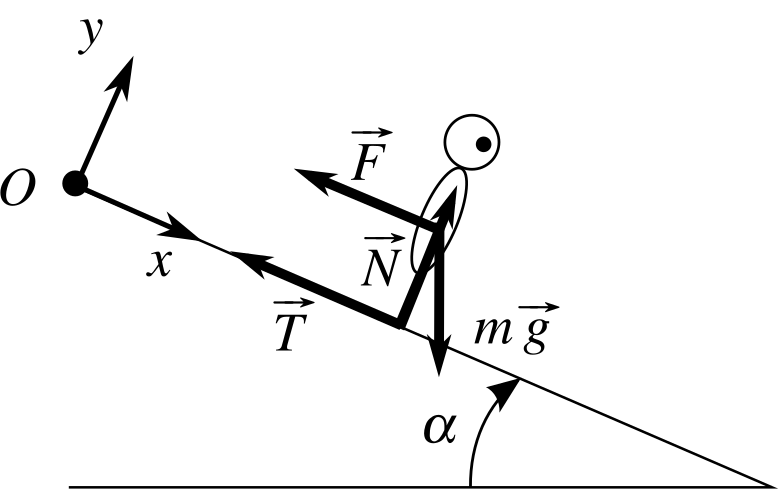
\includegraphics[width=.9\linewidth]{ski_corr}
		\end{center}
		\vspace{-3cm}
	\end{minipage}\smallbreak
	\begin{itemize}
		\item[b]{BDF}~:
		      \[
			      \begin{array}{ll}
				      \textbf{Poids}                 & m\gf = mg(\sin\a\ux - \cos\a\uy) \\
				      \textbf{Réaction normale}      & \Nf = N\uy                       \\
				      \textbf{Réaction tangentielle} & \Tf = -T\ux =
				      -fN\ux                                                            \\
				      \textbf{Frottements}           & \Ff = -\lb\vf = -\lb\xp\ux
			      \end{array}
		      \]
		      Comme la skieuse glisse sur la piste, avec les lois du
		      frottement de \textsc{Coulomb}, on a
		      \[T = fN\]
		\item[b]{PFD}~:
		      \[
			      m\af = \Pf + \Nf + \Tf + \Ff
			      \Lra
			      \left\{
			      \begin{aligned}
				      m\xpp & = mg\sin\a - fN - \lb\xp \\
				      m\ypp & = -mg\cos\a + N
			      \end{aligned}
			      \right.
		      \]
	\end{itemize}
	Ainsi, comme il n'y a pas de mouvement sur $\uy$, $\ypp = 0$ et
	\[
		\boxed{N = mg\cos\a}
		\Ra
		\boxed{T = fN = fmg\cos\a}
	\]
}
\QR{%
	Calculer la vitesse $\vf(t)$ et la position $x(t)$ de la skieuse à
	chaque instant $t$.
}{%
	On réutilise la première équation en y injectant l'expression de $T$
	pour avoir~:
	\[
		\xpp + \frac{\lb}{m}\xp = g(\sin\a - f\cos\a)
	\]
	Avec $\vf = \xp(t)\ux$, on obtient une équation différentielle sur
	$v(t)$ que l'on résout en posant $\tau = m/\lb$ avec la solution
	homogène $A\exr^{-t/\tau}$ et la solution particulière $v_p$~:
	\[
		\vp(t) + \frac{v}{\tau} = g(\sin\a - f\cos\a)
		\Ra
		v = A\exr^{-t/\tau} + v_p
	\]
	et on trouve $v_p$ directement en remarquant que, par construction,
	$\vp_p = 0$ donc $v_p = g\tau(\sin\a - f\cos\a)$. En combinant on peut
	utiliser la condition initiale sur la vitesse~:
	\begin{gather*}
		v(t) = A\exr^{-t/\tau} + g\tau(\sin\a - f\cos\a)
		\shortintertext{Or,}
		\left.
		\begin{aligned}
			v(0) & = 0
			\\\Lra
			0    & = A + g\tau(\sin\a - f\cos\a)
			\\\Lra
			A    & = -g\tau(\sin\a - f\cos\a)
		\end{aligned}
		\right\}
		\quad\Ra\quad
		\boxed{v(t) = g\tau(\sin\a - f\cos\a)\left(1-\exr^{-t/\tau}\right)}
	\end{gather*}
	On trouve la position $x(t)$ en intégrant $v(t)$~:
	\begin{gather*}
		x(t) = g\tau(\sin\a - f\cos\a)\left(t + \tau\exr^{-t/\tau}\right) +
		B
		\shortintertext{Or,}
		\left.
		\begin{aligned}
			x(0) & = 0
			\\\Lra
			0    & = g\tau(\sin\a - f\cos\a)\left(0 + \tau\right) + B
			\\\Lra
			B    & = -g\tau^2(\sin\a - f\cos\a)
		\end{aligned}
		\right\}
		\quad\Ra\quad
		\boxed{x(t) =
			g\tau(\sin\a-f\cos\a)\left(t+\tau\left(\exr^{-t/\tau}-1\right)\right)}
	\end{gather*}
}
\QR{%
	Montrer que la skieuse atteint une vitesse limite $\vf_l$ et exprimer
	$\vf(t)$ et $\OM(t)$ en fonction de $\vf_l$.
}{%
	La vitesse limite est la solution particulière $v_p$~:
	\[\boxed{\vf_l = g\tau(\sin\a-f\cos\a)\ux}\]
	En effet, la présence de la force de frottements fluides dont la norme
	augmente avec la vitesse fait que la vitesse ne peut pas augmenter
	indéfiniment. La skieuse atteint une vitesse limite lorsque les
	frottement compensent la force motrice du mouvement. Ainsi,
	\[
		\boxed{\vf(t) = v_l\left(1-\exr^{-t/\tau}\right)\ux}
		\qet
		\boxed{\OM(t) =
			v_l\left(t+\tau\left(\exr^{-t/\tau}-1\right)\right)\ux}
	\]
}
\QR{%
	Calculer $v_l = \norm{\vf_l}$ pour $\lambda = \SI{1}{kg.s^{-1}}$, $f =
		\num{0.9}$, $g = \SI{10}{m.s^{-1}}$, $m = \SI{65}{kg}$ et $\alpha =
		\ang{45;;}$.
}{%
	\begin{gather*}
		\boxed{v_l = \frac{mg}{\lb}(\sin\a-f\cos\a)}
		\qavec
		\left\{
		\begin{array}{rcl}
			m   & = & \SI{65}{kg}       \\
			g   & = & \SI{10}{m.s^{-2}} \\
			\lb & = & \SI{1}{kg.s^{-1}} \\
			\a  & = & \ang{45}          \\
			f   & = & \num{0.9}
		\end{array}
		\right.\\
		\AN
		\boxed{v_l = \SI{46}{m.s^{-1}}}
	\end{gather*}
	On remarque que la vitesse limite est une fonction affine du poids.
	Ainsi, le manque de représentation des femmes dans les sports d'hiver,
	souvent justifié par une moins bonne performance pure, est biaisé par la
	répartition moyenne de leurs tailles (et donc de leurs poids) plus
	faible que la répartition moyenne des tailles (et donc poids) des
	hommes, rendant \underline{pour certains} leurs records moins
	impressionnants.
}
\QR{%
	Calculer littéralement et numériquement la date $t_1$ où la skieuse a
	une vitesse égale à $v_l/2$.
}{%
	\begin{gather*}
		\begin{aligned}
			v(t_1)                 & = \frac{v_l}{2}
			\\\Lra
			\frac{\cancel{v_l}}{2} & = \cancel{v_l}(1-\exr^{-t_t/\tau})
			\\\Lra
			\frac{1}{2}            & = 1-\exr^{-t_1/\tau}
			\\\Lra
			\exr^{-t_1/\tau}       & = \frac{1}{2}
		\end{aligned}
		\\\Lra
		\boxed{t_1 = \tau\ln2}
		\qavec
		\tau = \frac{m}{\lb}
		\qet
		\left\{
		\begin{array}{rcl}
			m   & = & \SI{65}{kg}       \\
			\lb & = & \SI{1}{kg.s^{-1}}
		\end{array}
		\right.\\
		\AN
		\boxed{t_1 = \SI{45}{s}}
	\end{gather*}
}
\QR{%
	À la date $t_1$, la skieuse chute. On néglige alors la résistance de
	l'air et on considère que le coefficient de frottements sur le sol est
	multiplié par 10. Calculer la distance parcourue par la skieuse avant
	qu'elle ne s'arrête.
}{%
	En tombant à $t=t_1$, la skieuse a pour vitesse $v_l/2$. L'équation du
	mouvement sur $\uy$ ne change pas de forme, mais on multiplie $f$ par
	10, donc $T=10fmg$. Ainsi, en posant $t'=t-t_1$, en projection sur $\ux$
	et en négligeant $\lb$,
	\begin{gather*}
		\xpp(t') = g(\sin\a-10f\cos\a)
		\Ra
		\xp(t') = gt'(\sin\a-10f\cos\a) + v_l/2
	\end{gather*}
	On trouve le temps d'arrêt $t'_a$ quand $\xp(t'_a) = 0$, soit
	\[t'_a = \frac{-v_l}{2g(\sin\a-10f\cos\a)}\]
	et la distance d'arrêt depuis le point de chute en intégrant $\xp(t')$
	puis en prenant $x(t'_a)$~:
	\begin{gather*}
		x(t') = \frac{1}{2}gt'^2(\sin\a-10f\cos\a) + \frac{v_lt'}{2}
		\\\Lra
		\boxed{x(t'_a) = - \frac{v_l{}^2}{8g(\sin\a-10f\cos\a)}}
		\qavec
		\left\{
		\begin{array}{rcl}
			v_l & = & \SI{46}{m.s^{-1}} \\
			g   & = & \SI{10}{m.s^{-1}} \\
			\a  & = & \ang{45}          \\
			f   & = & \num{0.9}
		\end{array}
		\right.\\
		\AN
		\boxed{x(t'_a) = \SI{4.7}{m}}
	\end{gather*}
}
\end{document}
